\documentclass[11pt,paper=a4,answers]{exam}
\usepackage{graphicx,lastpage}
\usepackage{upgreek}
\usepackage{censor}
\usepackage{gensymb}
\usepackage{amsmath}
\usepackage{multicol}
\usepackage{enumitem}
\usepackage{tasks}
\usepackage{adjustbox}
\usepackage{xcolor}
\usepackage{tfrupee}
\setlength{\voffset}{0.25in}
\usepackage{tabularx}
\newcolumntype{Y}{>{\centering\arraybackslash}X}
%==============================================================
% Customise Non-Essential Packages Below
% =============================================================
\usepackage[most]{tcolorbox}
\usepackage{eso-pic}
\usepackage{tikz}
\AddToShipoutPictureBG{%
\begin{tikzpicture}[remember picture,overlay]
\foreach \x in {-8,-4,0,4,8,12,16,20}
\foreach \y in {-8,-4,0,4,8,12,16,20} {
\node[opacity=0.05,rotate=45,anchor=center] at ([xshift=\x cm,yshift=\y cm]current page.center) {%
\begin{minipage}{2cm}
\centering
\includegraphics[width=2cm]{images/logo_black.png}\\
\small preppeo.com
\end{minipage}%
};
}
\end{tikzpicture}%
}
\printanswers

%==============================================================
% Customise Non-Essential Packages Above
% =============================================================
\definecolor{svgray}{rgb}{0.90, 0.90, 0.90}
\graphicspath{{images/}}

\usepackage[normalem]{ulem}
\renewcommand\ULthickness{1pt}   %%---> For changing thickness of underline
\setlength\ULdepth{3.5ex}%\maxdimen ---> For changing depth of underline
\renewcommand{\baselinestretch}{1}
\chead{
\includegraphics[scale=0.1,height=2cm ]{logo.png}
}
\pagestyle{empty}

\pagestyle{headandfoot}
\headrule
\cfoot{W: https://preppeo.com; M: +91-8130711689}

\begin{document}
%==============================================================
% Customise Question paper details below this
% =============================================================
\begin{center}
    \centering
    \renewcommand{\arraystretch}{1.5}
    \begin{tabularx}{\textwidth}{YYY}
    & \normalsize\bf{{\Large{{Quant}}}} & \\
    By Preppeo & \normalsize\bf{{sat\_lid\_010}} & SAT\\
    \normalsize{{\textbf{{Unit:}} Algebra}} & \normalsize{{\textbf{{Chapter:}} Linear inequalities in one or two variables}} & \normalsize{{\textbf{{Topic:}} Solving \& Graphing Inequalities}} \\
    \end{tabularx}
\end{center}
\par\noindent\rule{\textwidth}{1pt}
% =============================================================
% Customise Question paper details above this
% =============================================================

\begin{questions}
\pointsinrightmargin
\pointsdroppedatright
\marksnotpoints
\pointpoints{mark}{marks}
\pointformat{\boldmath\themarginpoints}
\bracketedpoints

% =============================================================
% Question Begin
% =============================================================


% ==========================================
% TOPIC: Linear Inequalities (SAT LID: 010)
% ==========================================

%Q: 1
% Category: Practice | Difficulty: Easy | Question Type: Multiple Choice
\question
A landscaping service that mows both lawns and parks can mow at most 12 locations per day. Which inequality represents this situation, where $L$ is the number of lawns and $P$ is the number of parks?
\begin{tasks}(2)
    \task $L + P \le 12$
    \task $L + P \ge 12$
    \task $L - P \le 12$
    \task $L - P \ge 12$
\end{tasks}

\begin{solution}
\textbf{Conceptual Explanation:} \\
The phrase "at most" indicates a maximum limit. In mathematical terms, this translates to the "less than or equal to" symbol ($\le$). The total count of locations is the sum of the two types of properties.

\vspace{10pt}
\textbf{Calculation and Logic:} \\
Total locations = (Number of lawns) + (Number of parks) \\
Total locations = $L + P$ \\
Constraint: Must be no more than 12. \\
Inequality: $L + P \le 12$

\vspace{15pt}
Answer: \colorbox{yellow!100}{A}
\end{solution}

%Q: 2
% Category: Practice | Difficulty: Medium | Question Type: Multiple Choice
\question
The shaded region shown represents solutions to an inequality. Which ordered pair $(x, y)$ is a solution to this inequality?

\begin{center}
\begin{tikzpicture}[scale=0.5]
    \draw[help lines, color=gray!30, step=1] (-5,-5) grid (5,5);
    \draw[->,thick] (-5.5,0) -- (5.5,0) node[right] {$x$};
    \draw[->,thick] (0,-5.5) -- (0,5.5) node[above] {$y$};
    \foreach \x in {-4,-2,2,4} \draw (\x,0.1) -- (\x,-0.1) node[below] {\tiny \x};
    \foreach \y in {-4,-2,2,4} \draw (0.1,\y) -- (-0.1,\y) node[left] {\tiny \y};
    
    \fill[gray, opacity=0.5] (1,5) -- (5,5) -- (5,-5) -- (3,-5) -- cycle;
    \draw[very thick] (1,5) -- (3,-5);
\end{tikzpicture}
\end{center}

\begin{tasks}(2)
    \task $(0, 0)$
    \task $(-2, 2)$
    \task $(4, 1)$
    \task $(1, -2)$
\end{tasks}

\begin{solution}
\textbf{Conceptual Explanation:} \\
A solution to a graphed inequality is any point that lies within the shaded region or on the boundary line (if the line is solid).

\vspace{10pt}
\textbf{Calculation and Logic:} \\
Checking the points: \\
$(0, 0)$ is to the left of the shaded region. \\
$(-2, 2)$ is far to the left in the unshaded region. \\
$(1, -2)$ is on the left side of the boundary. \\
$(4, 1)$ is clearly inside the gray shaded area to the right of the line.

\vspace{15pt}
Answer: \colorbox{yellow!100}{C}
\end{solution}

%Q: 3
% Category: Practice | Difficulty: Medium | Question Type: Multiple Choice
\question
A delivery van can carry a maximum weight of 3,500 pounds. The van currently holds a machine weighing 400 pounds. If the rest of the load consists of identical crates weighing 150 pounds each, what is the maximum number of crates, $n$, the van can carry?
\begin{tasks}(2)
    \task 20
    \task 21
    \task 23
    \task 24
\end{tasks}

\begin{solution}
\textbf{Conceptual Explanation:} \\
The total weight is composed of a fixed value (the machine) and a variable value (the crates). This sum must be less than or equal to the van's capacity.

\vspace{10pt}
\textbf{Calculation and Logic:} \\
Total Weight = $400 + 150n$ \\
Constraint: $400 + 150n \le 3,500$ \\
Subtract 400: $150n \le 3,100$ \\
Divide by 150: $n \le 20.67$ \\
Since $n$ must be a whole number of crates, the maximum is 20.

\vspace{15pt}
Answer: \colorbox{yellow!100}{A}
\end{solution}

%Q: 4
% Category: Practice | Difficulty: Medium | Question Type: Numeric Entry
\question
David is renting a jet ski. The rental fee is \$45 per hour plus a mandatory \$15 insurance fee. David wants to spend no more than \$160. If he can only rent the jet ski for a whole number of hours, what is the maximum number of hours he can rent it?

\begin{solution}
\textbf{Conceptual Explanation:} \\
We establish a linear inequality where the hourly rate is the slope and the insurance is the y-intercept.

\vspace{10pt}
\textbf{Calculation and Logic:} \\
Let $h$ be the number of hours. \\
Cost: $45h + 15 \le 160$ \\
$45h \le 145$ \\
Divide by 45: $h \le 3.22$ \\
The largest whole number satisfying this is 3.

\vspace{15pt}
Answer: \colorbox{yellow!100}{3}
\end{solution}

%Q: 5
% Category: Practice | Difficulty: Hard | Question Type: Multiple Choice
\question
A craft store manager is ordering $x$ canvases and $y$ sets of paint. The manager must order at least 15 items, but the total budget is capped at \$120. Canvases cost \$5 each and paint sets cost \$8 each. Which system of inequalities models this?
\begin{tasks}(2)
    \task $x + y \ge 15$; $5x + 8y \le 120$
    \task $x + y \le 15$; $5x + 8y \ge 120$
    \task $5x + 8y \ge 15$; $x + y \le 120$
    \task $x + y \ge 15$; $5x + 8y \ge 120$
\end{tasks}

\begin{solution}
\textbf{Conceptual Explanation:} \\
"At least 15 items" means the sum of items $x$ and $y$ must be $\ge 15$. "Capped at \$120" means the total cost must be $\le 120$.

\vspace{10pt}
\textbf{Calculation and Logic:} \\
Count Inequality: $x + y \ge 15$ \\
Cost Inequality: (Price of $x \cdot x$) + (Price of $y \cdot y$) $\le$ Budget \\
$5x + 8y \le 120$

\vspace{15pt}
Answer: \colorbox{yellow!100}{A}
\end{solution}

%Q: 6
% Category: Practice | Difficulty: Hard | Question Type: Multiple Choice
\question
The average annual heating cost for a house is \$3,200. A new insulation system costs \$18,000 to install, after which the heating cost is estimated to drop to \$1,900 per year. Which inequality finds $t$, the years after which the total savings exceed the installation cost?
\begin{tasks}(1)
    \task $18,000 > (3,200 - 1,900)t$
    \task $18,000 < (3,200 - 1,900)t$
    \task $18,000 - 3,200 > 1,900t$
    \task $18,000 > \frac{3,200}{1,900}t$
\end{tasks}

\begin{solution}
\textbf{Conceptual Explanation:} \\
Savings per year is the difference between the old cost and the new cost. For total savings to "exceed" cost, (Savings $\times$ Time) must be greater than the installation price.

\vspace{10pt}
\textbf{Calculation and Logic:} \\
Annual Savings = $3,200 - 1,900$ \\
Total Savings over $t$ years = $(3,200 - 1,900)t$ \\
We want: Savings $>$ Cost \\
$(3,200 - 1,900)t > 18,000$, which is equivalent to $18,000 < (3,200 - 1,900)t$.

\vspace{15pt}
Answer: \colorbox{yellow!100}{B}
\end{solution}

%Q: 7
% Category: Practice | Difficulty: Medium | Question Type: Multiple Choice
\question
Which of the following ordered pairs $(x, y)$ satisfies the system below?
\[ y \le 2x + 3 \]
\[ x - y > 2 \]
\begin{tasks}(2)
    \task $(0, 0)$
    \task $(4, 1)$
    \task $(-2, -1)$
    \task $(1, 5)$
\end{tasks}

\begin{solution}
\textbf{Conceptual Explanation:} \\
An ordered pair is a solution if it makes BOTH inequalities true when substituted.

\vspace{10pt}
\textbf{Calculation and Logic:} \\
Test $(4, 1)$: \\
1) $1 \le 2(4) + 3 \Rightarrow 1 \le 11$ (True) \\
2) $4 - 1 > 2 \Rightarrow 3 > 2$ (True) \\
Since both are true, $(4, 1)$ is a solution.

\vspace{15pt}
Answer: \colorbox{yellow!100}{B}
\end{solution}

%Q: 8
% Category: Practice | Difficulty: Medium | Question Type: Multiple Choice
\question
A sea turtle travels 45 to 52 miles per day. Which inequality represents the estimated total miles, $m$, the turtle travels in 12 days?
\begin{tasks}(2)
    \task $45 + 12 \le m \le 52 + 12$
    \task $(45)(12) \le m \le (52)(12)$
    \task $45 \le m/12 \le 52$
    \task Both B and C
\end{tasks}

\begin{solution}
\textbf{Conceptual Explanation:} \\
To find the range over multiple days, we multiply the daily minimum and maximum by the number of days.

\vspace{10pt}
\textbf{Calculation and Logic:} \\
Minimum: $45 \times 12$ \\
Maximum: $52 \times 12$ \\
Range: $(45)(12) \le m \le (52)(12)$. \\
Note that dividing by 12 (Option C) also results in the daily speed, so B and C are mathematically equivalent.

\vspace{15pt}
Answer: \colorbox{yellow!100}{D}
\end{solution}

%Q: 9
% Category: Practice | Difficulty: Hard | Question Type: Multiple Choice
\question
The shaded region represents the solutions to which inequality?

\begin{center}
\begin{tikzpicture}[scale=0.5]
    \draw[help lines, color=gray!30, step=1] (-2,-8) grid (10,2);
    \draw[->,thick] (-2,0) -- (10,0) node[right] {$x$};
    \draw[->,thick] (0,-8) -- (0,2) node[above] {$y$};
    \fill[gray, opacity=0.4] (-2, -8) -- (10,0) -- (10,2) -- (-2,2) -- cycle;
    \draw[very thick] (-2, -8) -- (10,0);
\end{tikzpicture}
\end{center}

\begin{tasks}(2)
    \task $y \ge \frac{2}{3}x - 6.67$
    \task $y \le \frac{2}{3}x - 6.67$
    \task $y \ge x - 8$
    \task $y \le x - 8$
\end{tasks}

\begin{solution}
\textbf{Conceptual Explanation:} \\
Determine the y-intercept ($b$) and slope ($m$) of the line, then check if shading is above ($\ge$) or below ($\le$).

\vspace{10pt}
\textbf{Calculation and Logic:} \\
The line crosses the x-axis at $10$ and y-axis at approximately $-6.67$. \\
Slope $m = \frac{0 - (-6.67)}{10 - 0} = 0.667 = \frac{2}{3}$. \\
Shading is above the line. \\
Inequality: $y \ge \frac{2}{3}x - 6.67$.

\vspace{15pt}
Answer: \colorbox{yellow!100}{A}
\end{solution}

%Q: 10
% Category: Practice | Difficulty: Hard | Question Type: Numeric Entry
\question
Sarah earns \$12 per hour for the first 15 hours. Then she gets a raise to \$15 per hour. She saves 80\% of her earnings. What is the least number of additional hours she must work to save at least \$360?

\begin{solution}
\textbf{Conceptual Explanation:} \\
We must calculate her initial earnings, then determine the remaining amount needed, adjusting for her 80\% savings rate.

\vspace{10pt}
\textbf{Calculation and Logic:} \\
Initial Pay: $15 \text{ hours} \times \$12 = \$180$ \\
To save \$360 at an 80\% rate, she needs total pre-tax earnings ($E$): \\
$0.80E = 360 \Rightarrow E = 450$ \\
Earnings remaining needed: $450 - 180 = 270$ \\
Additional hours ($h$): $15h = 270 \Rightarrow h = 18$

\vspace{15pt}
Answer: \colorbox{yellow!100}{18}
\end{solution}

%Q: 11
% Category: Practice | Difficulty: Easy | Question Type: Multiple Choice
\question
A local library that lends both hardcovers and paperbacks can process at most 25 returns per hour. Which inequality represents this situation, where $c$ is the number of hardcovers and $p$ is the number of paperbacks?
\begin{tasks}(2)
    \task $c + p \le 25$
    \task $c + p \ge 25$
    \task $c - p \le 25$
    \task $c - p \ge 25$
\end{tasks}

\begin{solution}
\textbf{Conceptual Explanation:} \\
In SAT word problems, the phrase "at most" translates to the mathematical symbol $\le$. This indicates a limit that can be reached but not exceeded.

\vspace{10pt}
\textbf{Calculation and Logic:} \\
The total number of returns is the sum of the two types of books ($c$ and $p$). \\
Total returns = $c + p$ \\
Since the maximum is 25, the sum must be less than or equal to 25. \\
Inequality: $c + p \le 25$

\vspace{15pt}
Answer: \colorbox{yellow!100}{A}
\end{solution}

%Q: 12
% Category: Practice | Difficulty: Medium | Question Type: Multiple Choice
\question
The shaded region shown represents solutions to an inequality. Which ordered pair $(x, y)$ is a solution to this inequality?

\begin{center}
\begin{tikzpicture}[scale=0.6]
    \draw[help lines, color=gray!30, step=1] (-5,-5) grid (5,5);
    \draw[->,thick] (-5.5,0) -- (5.5,0) node[right] {$x$};
    \draw[->,thick] (0,-5.5) -- (0,5.5) node[above] {$y$};
    \foreach \x in {-4,-2,2,4} \draw (\x,0.1) -- (\x,-0.1) node[below] {\tiny \x};
    \foreach \y in {-4,-2,2,4} \draw (0.1,\y) -- (-0.1,\y) node[left] {\tiny \y};
    
    \fill[gray, opacity=0.5] (-5,3) -- (5,-2) -- (5,5) -- (-5,5) -- cycle;
    \draw[very thick] (-5,3) -- (5,-2);
\end{tikzpicture}
\end{center}

\begin{tasks}(2)
    \task $(0, -2)$
    \task $(-4, 0)$
    \task $(0, 4)$
    \task $(2, -3)$
\end{tasks}

\begin{solution}
\textbf{Conceptual Explanation:} \\
A point is a solution to a graphed inequality if it falls within the shaded region. We test each option by finding its location on the coordinate plane relative to the shaded area.

\vspace{10pt}
\textbf{Calculation and Logic:} \\
Checking the points: \\
$(0, -2)$ is below the boundary line in the white region. \\
$(-4, 0)$ is below the boundary line in the white region. \\
$(2, -3)$ is below the boundary line in the white region. \\
$(0, 4)$ is clearly above the line $y = -0.5x + 0.5$ and inside the shaded area.

\vspace{15pt}
Answer: \colorbox{yellow!100}{C}
\end{solution}

%Q: 13
% Category: Practice | Difficulty: Medium | Question Type: Multiple Choice
\question
A freight elevator has a maximum weight capacity of 2,800 pounds. A pallet weighing 300 pounds is already on the elevator. If the remaining capacity is filled with boxes that weigh 40 pounds each, what is the maximum number of boxes the elevator can safely carry?
\begin{tasks}(2)
    \task 60
    \task 62
    \task 63
    \task 70
\end{tasks}

\begin{solution}
\textbf{Conceptual Explanation:} \\
The total weight is the sum of the constant (the pallet) and the variable (the number of boxes multiplied by their unit weight). This sum cannot exceed the capacity.

\vspace{10pt}
\textbf{Calculation and Logic:} \\
Let $b$ be the number of boxes. \\
Inequality: $300 + 40b \le 2,800$ \\
Subtract 300: $40b \le 2,500$ \\
Divide by 40: $b \le 62.5$ \\
Since you cannot have half a box, the maximum whole number is 62.

\vspace{15pt}
Answer: \colorbox{yellow!100}{B}
\end{solution}

%Q: 14
% Category: Practice | Difficulty: Medium | Question Type: Numeric Entry
\question
Julia is renting a bicycle. The cost is \$12 per hour, plus a one-time \$8 helmet fee. Julia wants to spend no more than \$50 for the rental. If the bicycle is available only for a whole number of hours, what is the maximum number of hours for which Julia can rent the bicycle?

\begin{solution}
\textbf{Conceptual Explanation:} \\
This is a standard "no more than" problem, requiring a $\le$ inequality. We solve for the variable $h$ and round down to the nearest integer.

\vspace{10pt}
\textbf{Calculation and Logic:} \\
Let $h$ represent hours. \\
Cost: $12h + 8 \le 50$ \\
$12h \le 42$ \\
Divide by 12: $h \le 3.5$ \\
Because Julia can only rent for whole hours, the maximum is 3.

\vspace{15pt}
Answer: \colorbox{yellow!100}{3}
\end{solution}

%Q: 15
% Category: Practice | Difficulty: Hard | Question Type: Multiple Choice
\question
A high school club is buying $x$ pizzas and $y$ cases of soda for a party. The club must buy at least 12 items total, but the cost must not exceed \$150. If pizzas cost \$10 each and soda cases cost \$6 each, which system of inequalities models this?
\begin{tasks}(2)
    \task $x + y \le 12$; $10x + 6y \le 150$
    \task $x + y \ge 12$; $10x + 6y \ge 150$
    \task $x + y \ge 12$; $10x + 6y \le 150$
    \task $10x + 6y \ge 12$; $x + y \le 150$
\end{tasks}

\begin{solution}
\textbf{Conceptual Explanation:} \\
Systems of inequalities in SAT context usually involve a "count" constraint and a "cost" constraint. "At least" means $\ge$ and "not exceed" means $\le$.

\vspace{10pt}
\textbf{Calculation and Logic:} \\
Constraint 1 (Quantity): $x + y \ge 12$ \\
Constraint 2 (Budget): $10x + 6y \le 150$

\vspace{15pt}
Answer: \colorbox{yellow!100}{C}
\end{solution}

%Q: 16
% Category: Practice | Difficulty: Hard | Question Type: Multiple Choice
\question
A company's annual office supply expense is \$8,500. The office manager spends \$12,000 to switch to a paperless digital filing system. The manager estimates that the annual supply expense will then be \$1,200. Which inequality finds $n$, the number of years at which the cumulative savings will exceed the initial investment?
\begin{tasks}(1)
    \task $12,000 > (8,500 - 1,200)n$
    \task $12,000 < (8,500 - 1,200)n$
    \task $12,000 - 8,500 > 1,200n$
    \task $12,000 < \frac{8,500}{1,200}n$
\end{tasks}

\begin{solution}
\textbf{Conceptual Explanation:} \\
To "exceed" means to be greater than ($>$). We are comparing the investment cost to the annual savings multiplied by the number of years.

\vspace{10pt}
\textbf{Calculation and Logic:} \\
Annual Savings = (Old Cost - New Cost) = $8,500 - 1,200$ \\
Total Savings in $n$ years = $(8,500 - 1,200)n$ \\
Target: Savings $>$ Investment \\
$(8,500 - 1,200)n > 12,000$, which is the same as $12,000 < (8,500 - 1,200)n$.

\vspace{15pt}
Answer: \colorbox{yellow!100}{B}
\end{solution}

%Q: 17
% Category: Practice | Difficulty: Medium | Question Type: Multiple Choice
\question
Which of the following ordered pairs $(x, y)$ satisfies the system of inequalities below?
\[ y \le -2x + 4 \]
\[ x - y > 3 \]
\begin{tasks}(2)
    \task $(0, 0)$
    \task $(1, 2)$
    \task $(3, -2)$
    \task $(0, 5)$
\end{tasks}

\begin{solution}
\textbf{Conceptual Explanation:} \\
A solution must make both inequality statements true. We plug the $x$ and $y$ values from each option into both inequalities.

\vspace{10pt}
\textbf{Calculation and Logic:} \\
Test $(3, -2)$: \\
1) $-2 \le -2(3) + 4 \Rightarrow -2 \le -2$ (True) \\
2) $3 - (-2) > 3 \Rightarrow 5 > 3$ (True) \\
Because $(3, -2)$ satisfies both, it is a solution.

\vspace{15pt}
Answer: \colorbox{yellow!100}{C}
\end{solution}

%Q: 18
% Category: Practice | Difficulty: Medium | Question Type: Multiple Choice
\question
A migration model for monarch butterflies estimates they travel 65 to 80 miles per day. Which inequality represents the estimated total number of miles, $d$, a butterfly could travel in 14 days?
\begin{tasks}(2)
    \task $65 + 14 \le d \le 80 + 14$
    \task $(65)(14) \le d \le (80)(14)$
    \task $65 \le d + 14 \le 80$
    \task $65 \le 14d \le 80$
\end{tasks}

\begin{solution}
\textbf{Conceptual Explanation:} \\
If we know the range for one day, we find the range for $N$ days by multiplying both the lower and upper bounds by $N$.

\vspace{10pt}
\textbf{Calculation and Logic:} \\
Minimum distance = $65 \times 14$ \\
Maximum distance = $80 \times 14$ \\
Total miles $d$ must be between these two values: $(65)(14) \le d \le (80)(14)$.

\vspace{15pt}
Answer: \colorbox{yellow!100}{B}
\end{solution}

%Q: 19
% Category: Practice | Difficulty: Medium | Question Type: Multiple Choice
\question
The shaded region shown represents the solutions to which inequality?

\begin{center}
\begin{tikzpicture}[scale=0.5]
    \draw[help lines, color=gray!30, step=1] (-1,-10) grid (11,1);
    \draw[->,thick] (-1,0) -- (11,0) node[right] {$x$};
    \draw[->,thick] (0,-10) -- (0,1) node[above] {$y$};
    \fill[gray, opacity=0.4] (-1, -10) -- (11,-2) -- (11,1) -- (-1,1) -- cycle;
    \draw[very thick] (-1, -10) -- (11,-2);
\end{tikzpicture}
\end{center}

\begin{tasks}(2)
    \task $y \le \frac{2}{3}x - 9.33$
    \task $y \ge \frac{2}{3}x - 9.33$
    \task $y \ge x - 10$
    \task $y \le x - 10$
\end{tasks}

\begin{solution}
\textbf{Conceptual Explanation:} \\
The boundary line's equation is $y = mx + b$. We find the y-intercept ($b$) and use a second point to find slope ($m$). Since shading is above the line, we use $\ge$.

\vspace{10pt}
\textbf{Calculation and Logic:} \\
The line passes through $(0, -9.33)$ and $(14, 0)$. \\
Slope $m = \frac{0 - (-9.33)}{14 - 0} = \frac{2}{3}$. \\
Shading is above the line. \\
Inequality: $y \ge \frac{2}{3}x - 9.33$.

\vspace{15pt}
Answer: \colorbox{yellow!100}{B}
\end{solution}

%Q: 20
% Category: Practice | Difficulty: Hard | Question Type: Multiple Choice
\question
Marcus is working a summer job. He earns \$15 per hour for the first 20 hours. For any hours over 20, he earns \$18 per hour. If Marcus saves 75\% of his total earnings, what is the least number of overtime hours he must work to save at least \$450?
\begin{tasks}(2)
    \task 17
    \task 12
    \task 8
    \task 6
\end{tasks}

\begin{solution}
\textbf{Conceptual Explanation:} \\
We first find how much total he needs to earn to save \$450, then calculate the earnings from his base hours, and finally find the required overtime hours.

\vspace{10pt}
\textbf{Calculation and Logic:} \\
Let $E$ be total earnings. $0.75E = 450 \Rightarrow E = 600$. \\
Base Earnings = $20 \times 15 = 300$. \\
Remaining needed = $600 - 300 = 300$. \\
Overtime hours $x$: $18x = 300 \Rightarrow x = 16.67$. \\
Least whole number of hours is 17.

\vspace{15pt}
Answer: \colorbox{yellow!100}{A}
\end{solution}

%Q: 21
% Category: Practice | Difficulty: Easy | Question Type: Multiple Choice
\question
A gym allows a maximum of 40 members inside at one time. If $s$ represents students and $a$ represents adults, which inequality represents the capacity?
\begin{tasks}(2)
    \task $s + a \le 40$
    \task $s + a \ge 40$
    \task $s - a \le 40$
    \task $s + a < 40$
\end{tasks}

\begin{solution}
\textbf{Conceptual Explanation:} \\
"Maximum" implies that 40 is the limit. The sum can be equal to 40 or less than 40.

\vspace{15pt}
Answer: \colorbox{yellow!100}{A}
\end{solution}

%Q: 22
% Category: Practice | Difficulty: Medium | Question Type: Numeric Entry
\question
A parking garage charges \$5 for the first hour and \$3 for each additional hour. A driver has a maximum budget of \$20. If the garage only charges for whole hours, what is the maximum number of total hours the driver can park?

\begin{solution}
\textbf{Conceptual Explanation:} \\
Note that the first hour is a fixed \$5, and the \$3 rate only applies to hours *after* the first.

\vspace{10pt}
\textbf{Calculation and Logic:} \\
Let $x$ be the number of additional hours. \\
Total Cost: $5 + 3x \le 20$ \\
$3x \le 15 \Rightarrow x \le 5$. \\
Total hours = 1 (first hour) + 5 (additional hours) = 6.

\vspace{15pt}
Answer: \colorbox{yellow!100}{6}
\end{solution}

%Q: 23
% Category: Practice | Difficulty: Hard | Question Type: Multiple Choice
\question
A farmer is planting $x$ acres of corn and $y$ acres of wheat. He has at least 50 acres of land available, but his seed budget is \$2,000. Corn seeds cost \$40 per acre and wheat seeds cost \$30 per acre. Which system models this?
\begin{tasks}(2)
    \task $x + y \ge 50$; $40x + 30y \le 2,000$
    \task $x + y \le 50$; $40x + 30y \le 2,000$
    \task $40x + 30y \ge 50$; $x + y \le 2,000$
    \task $x + y \ge 50$; $40x + 30y \ge 2,000$
\end{tasks}

\begin{solution}
\textbf{Logic:} \\
Acreage constraint: $x + y \ge 50$. Budget constraint: $40x + 30y \le 2,000$.

\vspace{15pt}
Answer: \colorbox{yellow!100}{A}
\end{solution}

%Q: 24
% Category: Practice | Difficulty: Medium | Question Type: Multiple Choice
\question
A car travels between 55 and 65 miles per hour. Which inequality represents the distance $d$ it could travel in 3 hours?
\begin{tasks}(2)
    \task $55 \times 3 \le d \le 65 \times 3$
    \task $55 + 3 \le d \le 65 + 3$
    \task $55 \le 3d \le 65$
    \task $d/3 \le 55$
\end{tasks}

\begin{solution}
\textbf{Logic:} \\
Multiply both bounds of the hourly rate by 3 hours.

\vspace{15pt}
Answer: \colorbox{yellow!100}{A}
\end{solution}

%Q: 25
% Category: Practice | Difficulty: Hard | Question Type: Multiple Choice
\question
Which ordered pair $(x, y)$ is a solution to the system: $y > 2x - 4$ and $y < -x + 5$?
\begin{tasks}(2)
    \task $(4, 0)$
    \task $(0, 0)$
    \task $(5, 5)$
    \task $(0, 6)$
\end{tasks}

\begin{solution}
\textbf{Logic:} \\
Test $(0, 0)$: \\
1) $0 > 2(0) - 4 \Rightarrow 0 > -4$ (True) \\
2) $0 < -0 + 5 \Rightarrow 0 < 5$ (True)

\vspace{15pt}
Answer: \colorbox{yellow!100}{B}
\end{solution}

%Q: 26
% Category: Practice | Difficulty: Medium | Question Type: Multiple Choice
\question
Which of the following describes the solution set to the system of inequalities below?
\[ y > 3x + 2 \]
\[ y < 3x - 4 \]
\begin{tasks}(1)
    \task A narrow strip between two parallel lines.
    \task All points in the $xy$-plane.
    \task No solution.
    \task A single point of intersection.
\end{tasks}

\begin{solution}
\textbf{Conceptual Explanation:} \\
In a system of inequalities, the solution set is the overlap of the two individual regions. If the boundary lines are parallel and the shaded regions face away from each other, there is no overlap.

\vspace{10pt}
\textbf{Calculation and Logic:} \\
Both lines have the same slope ($m=3$), meaning they are parallel. 
The first inequality shades everything ABOVE $y = 3x + 2$. 
The second inequality shades everything BELOW $y = 3x - 4$. 
Since the "above" region of the higher line and the "below" region of the lower line never touch, there is no common area.

\vspace{15pt}
Answer: \colorbox{yellow!100}{C}
\end{solution}

%Q: 27
% Category: Practice | Difficulty: Hard | Question Type: Numeric Entry
\question
For a system of inequalities, $y \ge 2x + b$ and $y \le 2x + c$. If $b = -5$ and $c = -5$, how many integer values of $y$ exist for the point where $x = 4$?

\begin{solution}
\textbf{Conceptual Explanation:} \\
When the two boundary lines are the same but the inequalities face opposite directions (and include the "equal to" component), the solution set is restricted to the boundary line itself.

\vspace{10pt}
\textbf{Calculation and Logic:} \\
Substitute $b$ and $c$:
1) $y \ge 2x - 5$
2) $y \le 2x - 5$
The only way $y$ can be both $\ge$ and $\le$ the same value is if $y$ equals that value.
At $x = 4$:
$y = 2(4) - 5 = 3$
There is exactly one integer value for $y$, which is 3.

\vspace{15pt}
Answer: \colorbox{yellow!100}{1}
\end{solution}

%Q: 28
% Category: Practice | Difficulty: Medium | Question Type: Multiple Choice
\question
Which of the following systems of inequalities has the entire $xy$-plane as its solution set?
\begin{tasks}(1)
    \task $y > x$ and $y < x$
    \task $y \ge x$ and $y \le x$
    \task $y > x - 5$ or $y < x + 5$
    \task $y > 5$ and $x > 5$
\end{tasks}

\begin{solution}
\textbf{Conceptual Explanation:} \\
The word "or" in a compound inequality (union) means the solution is any point that satisfies at least one of the inequalities.

\vspace{10pt}
\textbf{Calculation and Logic:} \\
In Option C, $y > x - 5$ covers everything above the lower line. $y < x + 5$ covers everything below the higher line. Because these two regions overlap and extend to infinity in opposite directions, every single point in the plane satisfies at least one of them.

\vspace{15pt}
Answer: \colorbox{yellow!100}{C}
\end{solution}

%Q: 29
% Category: Practice | Difficulty: Hard | Question Type: Numeric Entry
\question
A system of inequalities is given by $y > 4x + 10$ and $y < 4x + k$. If the system has no solution, what is the maximum possible integer value for $k$?

\begin{solution}
\textbf{Conceptual Explanation:} \\
For "no solution" with parallel lines, the region shaded "above" the first line must not overlap the region shaded "below" the second line. This happens if the second line is below or equal to the first line.

\vspace{10pt}
\textbf{Calculation and Logic:} \\
The first line is $y = 4x + 10$ (shaded above). 
The second line is $y = 4x + k$ (shaded below). 
If $k \le 10$, the area below $k$ and the area above 10 will never meet. 
The largest integer $k$ that maintains no overlap is 10.

\vspace{15pt}
Answer: \colorbox{yellow!100}{10}
\end{solution}

%Q: 30
% Category: Practice | Difficulty: Medium | Question Type: Multiple Choice
\question
An inequality is graphed such that the boundary line passes through $(0, -4)$ and $(2, 0)$, and the shading is below the line. Which of the following is the inequality?
\begin{tasks}(2)
    \task $y \le 2x - 4$
    \task $y \ge 2x - 4$
    \task $y \le -2x - 4$
    \task $y \ge -2x - 4$
\end{tasks}

\begin{solution}
\textbf{Calculation and Logic:} \\
Slope $m = \frac{0 - (-4)}{2 - 0} = \frac{4}{2} = 2$. \\
Y-intercept $b = -4$. \\
Boundary line: $y = 2x - 4$. \\
Shading below indicates $\le$.

\vspace{15pt}
Answer: \colorbox{yellow!100}{A}
\end{solution}

%Q: 31
% Category: Practice | Difficulty: Medium | Question Type: Multiple Choice
\question
Which point $(x, y)$ satisfies the inequality $3x - 4y > 12$?
\begin{tasks}(2)
    \task $(4, 0)$
    \task $(0, -3)$
    \task $(6, 1)$
    \task $(2, -2)$
\end{tasks}

\begin{solution}
\textbf{Calculation and Logic:} \\
A: $3(4) - 4(0) = 12$. $12 > 12$ (False). \\
B: $3(0) - 4(-3) = 12$. $12 > 12$ (False). \\
C: $3(6) - 4(1) = 18 - 4 = 14$. $14 > 12$ (True).

\vspace{15pt}
Answer: \colorbox{yellow!100}{C}
\end{solution}

%Q: 32
% Category: Practice | Difficulty: Medium | Question Type: Multiple Choice
\question
A system of inequalities is graphed below. Which region contains the solution set?

\begin{center}
\begin{tikzpicture}[scale=0.6]
    \draw[->] (-3,0) -- (3,0) node[right] {$x$};
    \draw[->] (0,-3) -- (0,3) node[above] {$y$};
    \draw[thick] (-3,1) -- (3,-2) node[right] {$l_1$};
    \draw[thick] (-1,-3) -- (2,3) node[right] {$l_2$};
    \node at (2,0) {I};
    \node at (0,2) {II};
    \node at (-2,0) {III};
    \node at (0,-2) {IV};
\end{tikzpicture}
\end{center}

If the system is $y > l_1$ and $x > 0.5$, which region is correct?
\begin{tasks}(4)
    \task Region I
    \task Region II
    \task Region III
    \task Region IV
\end{tasks}

\begin{solution}
\textbf{Calculation and Logic:} \\
Region I is to the right of the vertical-ish line ($x > 0.5$) and above the horizontal-ish line ($y > l_1$).

\vspace{15pt}
Answer: \colorbox{yellow!100}{A}
\end{solution}

%Q: 33
% Category: Practice | Difficulty: Hard | Question Type: Numeric Entry
\question
A theater sells tickets for \$20 and \$30. The theater must sell at least 100 tickets and wants to make more than \$2,600. What is the minimum number of \$30 tickets they can sell to meet both goals?

\begin{solution}
\textbf{Calculation and Logic:} \\
$x + y \ge 100 \Rightarrow x = 100 - y$ \\
$20x + 30y > 2,600$ \\
$20(100 - y) + 30y > 2,600$ \\
$2,000 - 20y + 30y > 2,600$ \\
$10y > 600 \Rightarrow y > 60$. \\
The minimum integer is 61.

\vspace{15pt}
Answer: \colorbox{yellow!100}{61}
\end{solution}

%Q: 34
% Category: Practice | Difficulty: Medium | Question Type: Multiple Choice
\question
$y < x + 5$. If $x$ increases by 2, what must happen to the maximum possible value of $y$?
\begin{tasks}(1)
    \task It decreases by 2.
    \task It increases by 2.
    \task It remains the same.
    \task It increases by 5.
\end{tasks}

\begin{solution}
\textbf{Logic:} \\
If $y_{max} \approx x + 5$, then $(x+2) + 5 = (x+5) + 2$. The bound increases by 2.

\vspace{15pt}
Answer: \colorbox{yellow!100}{B}
\end{solution}

%Q: 35
% Category: Practice | Difficulty: Easy | Question Type: Multiple Choice
\question
The inequality $x \ge -3$ is graphed in the $xy$-plane. Which describes the shading?
\begin{tasks}(1)
    \task Above a horizontal line.
    \task Below a horizontal line.
    \task To the left of a vertical line.
    \task To the right of a vertical line.
\end{tasks}

\begin{solution}
\textbf{Logic:} \\
$x = -3$ is a vertical line. $x \ge -3$ means all $x$-values greater than -3, which are to the right.

\vspace{15pt}
Answer: \colorbox{yellow!100}{D}
\end{solution}

%Q: 36
% Category: Practice | Difficulty: Medium | Question Type: Numeric Entry
\question
A student needs an average of at least 90 on two tests. On the first test, she scored 84. What is the minimum score she needs on the second test?

\begin{solution}
\textbf{Logic:} \\
$(84 + x)/2 \ge 90$ \\
$84 + x \ge 180 \Rightarrow x \ge 96$.

\vspace{15pt}
Answer: \colorbox{yellow!100}{96}
\end{solution}

%Q: 37
% Category: Practice | Difficulty: Hard | Question Type: Multiple Choice
\question
In a system of inequalities, the solution region is a triangle. Which of the following could be the system?
\begin{tasks}(1)
    \task $x > 0, y > 0, x + y < 5$
    \task $x > 0, y > 0, y > x + 5$
    \task $x > 5, x < 2$
    \task $y > x, y > -x$
\end{tasks}

\begin{solution}
\textbf{Logic:} \\
Option A is bounded by the $x$-axis, $y$-axis, and the line $x+y=5$, forming a triangle in the first quadrant.

\vspace{15pt}
Answer: \colorbox{yellow!100}{A}
\end{solution}

%Q: 38
% Category: Practice | Difficulty: Medium | Question Type: Multiple Choice
\question
Which inequality is equivalent to $-2y + 4x < 10$?
\begin{tasks}(2)
    \task $y < 2x - 5$
    \task $y > 2x - 5$
    \task $y < -2x + 5$
    \task $y > -2x + 5$
\end{tasks}

\begin{solution}
\textbf{Logic:} \\
$-2y < -4x + 10$ \\
Divide by -2 (flip the inequality): $y > 2x - 5$.

\vspace{15pt}
Answer: \colorbox{yellow!100}{B}
\end{solution}

%Q: 39
% Category: Practice | Difficulty: Medium | Question Type: Multiple Choice
\question
If $(k, 2k)$ is a solution to $x + y \le 12$, what is the maximum value of $k$?
\begin{tasks}(2)
    \task 3
    \task 4
    \task 6
    \task 12
\end{tasks}

\begin{solution}
\textbf{Logic:} \\
$k + 2k \le 12 \Rightarrow 3k \le 12 \Rightarrow k \le 4$.

\vspace{15pt}
Answer: \colorbox{yellow!100}{B}
\end{solution}

%Q: 40
% Category: Practice | Difficulty: Hard | Question Type: Multiple Choice
\question
A system has inequalities $y \ge |x|$ and $y \le 4$. What is the area of the solution region?
\begin{tasks}(2)
    \task 8
    \task 16
    \task 32
    \task 4
\end{tasks}

\begin{solution}
\textbf{Logic:} \\
This forms a triangle with vertices $(0,0), (-4,4), (4,4)$. \\
Base = 8, Height = 4. Area = $0.5 \times 8 \times 4 = 16$.

\vspace{15pt}
Answer: \colorbox{yellow!100}{B}
\end{solution}

%Q: 41
% Category: Practice | Difficulty: Medium | Question Type: Numeric Entry
\question
If $y > 2x + 1$ and $y < 2x + 5$, how many integer values of $y$ are possible when $x = 0.5$?

\begin{solution}
\textbf{Logic:} \\
$y > 2(0.5) + 1 \Rightarrow y > 2$ \\
$y < 2(0.5) + 5 \Rightarrow y < 6$ \\
Integers: 3, 4, 5. Total = 3.

\vspace{15pt}
Answer: \colorbox{yellow!100}{3}
\end{solution}

%Q: 42
% Category: Practice | Difficulty: Hard | Question Type: Multiple Choice
\question
For which value of $a$ does the system $y > ax + 2$ and $y < 2x + 5$ have a solution region in the second quadrant?
\begin{tasks}(2)
    \task $a = 2$
    \task $a = 5$
    \task $a = -1$
    \task All of the above
\end{tasks}

\begin{solution}
\textbf{Logic:} \\
The second quadrant is where $x < 0$ and $y > 0$. Both boundaries have positive y-intercepts, so regions above/near these intercepts will always include parts of the second quadrant.

\vspace{15pt}
Answer: \colorbox{yellow!100}{D}
\end{solution}

%Q: 43
% Category: Practice | Difficulty: Medium | Question Type: Multiple Choice
\question
$x + y > 10$. If $x < 4$, what is true about $y$?
\begin{tasks}(1)
    \task $y > 6$
    \task $y < 6$
    \task $y > 10$
    \task $y < 14$
\end{tasks}

\begin{solution}
\textbf{Logic:} \\
$y > 10 - x$. If $x$ is at its maximum (almost 4), $y$ must be at least $10 - 4 = 6$. So $y$ must be greater than 6.

\vspace{15pt}
Answer: \colorbox{yellow!100}{A}
\end{solution}

%Q: 44
% Category: Practice | Difficulty: Hard | Question Type: Numeric Entry
\question
How many points $(x, y)$ with integer coordinates satisfy $x > 0, y > 0,$ and $x + y < 4$?

\begin{solution}
\textbf{Logic:} \\
Points: $(1, 1), (1, 2), (2, 1)$. Total = 3.

\vspace{15pt}
Answer: \colorbox{yellow!100}{3}
\end{solution}

%Q: 45
% Category: Practice | Difficulty: Medium | Question Type: Multiple Choice
\question
The solution to $y < mx + b$ does not include any points in the first quadrant. What must be true about $m$ and $b$?
\begin{tasks}(2)
    \task $m > 0, b > 0$
    \task $m < 0, b < 0$
    \task $m > 0, b < 0$
    \task $m < 0, b > 0$
\end{tasks}

\begin{solution}
\textbf{Logic:} \\
For a line to stay out of the first quadrant while shading below, it must have a negative slope and a negative y-intercept.

\vspace{15pt}
Answer: \colorbox{yellow!100}{B}
\end{solution}

%Q: 46
% Category: Practice | Difficulty: Medium | Question Type: Multiple Choice
\question
$y \ge x + 2$ and $y \le x + 2$. This system describes:
\begin{tasks}(2)
    \task No points
    \task A single point
    \task A line
    \task A shaded region
\end{tasks}

\begin{solution}
\textbf{Logic:} \\
When $y$ is both $\ge$ and $\le$ the same expression, $y$ must equal that expression. $y = x + 2$ is a line.

\vspace{15pt}
Answer: \colorbox{yellow!100}{C}
\end{solution}

%Q: 47
% Category: Practice | Difficulty: Hard | Question Type: Multiple Choice
\question
If $y > x^2$ and $y < 4$, how many integer points $(x, y)$ are solutions?
\begin{tasks}(2)
    \task 3
    \task 5
    \task 6
    \task 7
\end{tasks}

\begin{solution}
\textbf{Logic:} \\
$x=0: y=1,2,3$ (3 pts) \\
$x=1: y=2,3$ (2 pts) \\
$x=-1: y=2,3$ (2 pts) \\
Total = 7.

\vspace{15pt}
Answer: \colorbox{yellow!100}{D}
\end{solution}

%Q: 48
% Category: Practice | Difficulty: Medium | Question Type: Numeric Entry
\question
$3x - y < 5$. If $(2, y)$ is a solution, what is the smallest integer value for $y$?

\begin{solution}
\textbf{Logic:} \\
$3(2) - y < 5 \Rightarrow 6 - y < 5 \Rightarrow 1 < y$. \\
Smallest integer strictly greater than 1 is 2.

\vspace{15pt}
Answer: \colorbox{yellow!100}{2}
\end{solution}

%Q: 49
% Category: Practice | Difficulty: Medium | Question Type: Multiple Choice
\question
$x + y > 5$ and $x + y < 5$. This system has:
\begin{tasks}(2)
    \task One solution
    \task Infinite solutions
    \task No solution
    \task A solution at $(2.5, 2.5)$
\end{tasks}

\begin{solution}
\textbf{Logic:} \\
A value cannot be strictly greater than and strictly less than 5 at the same time.

\vspace{15pt}
Answer: \colorbox{yellow!100}{C}
\end{solution}

%Q: 50
% Category: Practice | Difficulty: Hard | Question Type: Numeric Entry
\question
In the system $y > 2x + 10$ and $y < -x + 25$, what is the maximum possible integer $x$-coordinate for a solution?

\begin{solution}
\textbf{Logic:} \\
Set boundaries equal: $2x + 10 = -x + 25 \Rightarrow 3x = 15 \Rightarrow x = 5$. \\
Since the inequalities are strict ($<$ and $>$), $x$ must be less than 5. Max integer is 4.

\vspace{15pt}
Answer: \colorbox{yellow!100}{4}
\end{solution}

% =============================================================
% Question End
% =============================================================

\end{questions}
\begin{center}
\rule{.5\textwidth}{1pt}
\end{center}
\end{document}
